% ---------------------------------------------------------------------------- %
\subsection{Das R\"ontgen-Spektrum}
\label{subsec:rontgenSpektrum}
% ---------------------------------------------------------------------------- %

\begin{figure}[h!]
    \centering
    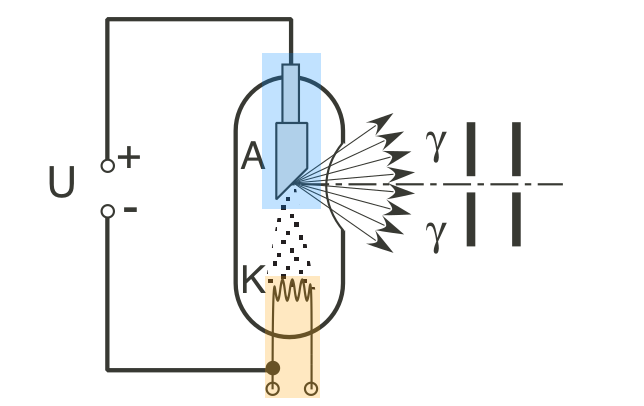
\includegraphics[width=0.5\textwidth]{images/rontgen-rohre.png}
    \caption{%
        R\"ontgen-R\"ohre,  schematisch. Gl\"uhkathode  K:  orange,  Anode  A:
        blau. \emph{Quelle}: Versuchsanleitung
    }
    \label{fig:rontgenRohre}
\end{figure}

R\"ontgen-Strahlung   entsteht    stets,   wenn   schnelle    Elektronen   auf
Materie  treffen,  z.B.  in   einem  Monitor  mit  Kathodenstrahl-R\"ohre. Sie
besteht   aus   einer   Gl\"uhkathode    \textbf{K}   (orange   in   Abbildung
\ref{fig:rontgenRohre})  und   einer  Anode  \textbf{A}  (blau   in  Abbildung
\ref{fig:rontgenRohre}). Eingeschlossen  ist das  Ganze in  einem vakuumierten
Glaskolben.

Die  Kathode  gibt  durch  ihre  Erhitzung Elektronen  ab,  welche  durch  das
Elektrische  Feld  zwischen  Kathode  und Anode  auf  die  Anode  beschleunigt
werden   (Spannung  zwischen   Kathode  und   Anode:  \"ublicherweise   einige
\SI{10}{\kilo\volt} bis  einige \SI{100}{\kilo\volt}, in diesem  Versuch liegt
sie  zwischen \SI{12}{\kilo\volt}  und \SI{35}{\kilo\volt}).   Beim Auftreffen
auf die Anode haben die Elektronen somit eine Energie von $E_k = e \cdot U$.

In der Anode  wird nun ein kleiner Teil (weniger  als \SI{1}{\percent}) dieser
Energie in R\"ontgenstrahlung  umgewandelt (der Rest geht in  die Anregung und
Ionisation der Metallatome der Anode).

Da  die abgegebene  R\"ontgenstrahlung  einigermassen isotrop  ist, wird  eine
Abschirmung  ben\"otigt, um  nicht  ziellos die  Umgebung zu  verstrahlen. Der
R\"ontgenstrahl wird weiter auf eine  nutzbar kleine Form reduziert, indem man
einen Bleikollimator benutzt.

Als  Anodenmaterial wird  normalerweise  ein Metall  mit  mittlerer bis  hoher
Ordnungszahl verwendet. In diesem Versuch kommen  Kupfer ($Z = 29$), Eisen ($Z
= 26$) und Molybd\"an ($Z = 42$) zum Einsatz.

\clearpage
Das R\"ontgen-Spektrum selbst besteht aus zwei Komponenten:
\begin{itemize}
    \item
        \textbf{Bremskontinuum:}    unspezifische   Form,    Einsatzpunkt   am
        kurzwelligen Ende ($\lambda_G$ in Abbildung \ref{fig:rontgenSpektrum})
        ist abh\"angig von der R\"ohrenspannung.
    \item
        \textbf{R\"ontgenlinien:}  diskrete,  vom  Anodenmaterial  abh\"angige
        Strahlung, unabh\"angig von der Spannung
\end{itemize}

\begin{figure}[h!]
    \centering
    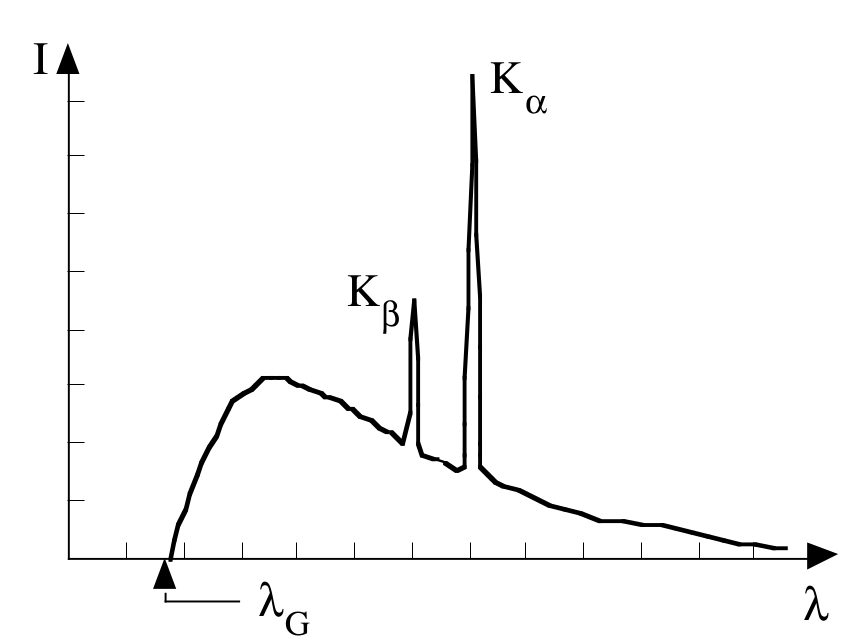
\includegraphics[width=0.5\textwidth]{images/rontgen-spektrum.png}
    \caption{%
        R\"ontgen-Spektrum. \emph{Quelle}: Versuchsanleitung
    }
    \label{fig:rontgenSpektrum}
\end{figure}

% ---------------------------------------------------------------------------- %
\subsubsection{Die Bremsstrahlung}
\label{subsubsec:bremsstrahlung}
% ---------------------------------------------------------------------------- %

Dringt ein Elektron von der Kathode in ein Atom der Anode ein und kommt in den
Einflussbereich des Coulomb-Feldes des Kerns, wird gem\"ass Quantentheorie ein
Photon $\gamma$ abgegeben.

Die Grenze der  k\"urzesten Wellenl\"ange $\lambda_G$, die  im Spektrum dieser
Photonen auftritt, beschreibt  die Situation, wenn ein  emittiertes Photon die
gesamte Energie eines einfallenden  Elektrons aufgenommen hat (zur Erinnerung:
k\"urzere  Wellenl\"ange  korrespondiert  mit  h\"oherer  Frequenz  und  somit
h\"oherer Energie eines  Photons). Da es unm\"oglich ist, mehr  Energie in ein
Photon zu transferieren,  als das einfallende Elektron  mitbringt, reisst dort
das Spektrum am linken Ende ab.

Die  maximale  Energie,  die  ein  emittiertes  R\"ontgen-Photon  haben  kann,
berechnet sich somit zu

\begin{equation}
    \label{eq:E_gamma_max}
    E_{\gamma,max} = e \cdot U
\end{equation}

mit der zugeh\"origen Wellenl\"ange:

\begin{equation}
    \label{eq:lambda_G}
    \lambda_G = \frac{h \cdot c}{e \cdot U}
\end{equation}

$h$  ist dabei  die Planck-Konstante,  $c$ die  Lichtgeschwindigkeit, $e$  die
Ladung eines Elektrons und $U$ die R\"ohrenspannung.


% ---------------------------------------------------------------------------- %
\subsubsection{Die charakteristische Strahlung}
\label{subsubsec:charaktStrahlung}
% ---------------------------------------------------------------------------- %

Die charakteristische Strahlung geht von den Atomen des Anodenmaterials selbst aus.
Sie besteht aus Photonen, die bei Elektronen\"uberg\"angen in der kernnahen Atomh\"ulle
abgegeben werden:

\begin{minipage}[c][][b]{0.585\textwidth}
    \begin{itemize}
        \item
            L-Schale $\rightarrow$ K-Schale: $K_\alpha$-Strahlung
        \item
            M-Schale $\rightarrow$ K-Schale: $K_\beta$-Strahlung
        \item
            M-, N-, O-Schale $\rightarrow$ L-Schale: $L$-Strahlung
    \end{itemize}

    Solche  \"Uberg\"ange werden  erm\"oglicht  durch  das herausschlagen  von
    Elektronen aus einer inneren Schalde (Elektronenstoss/Stossionisation oder
    Absorption von R\"ontgen-Strahlung/Photoionisation).

\end{minipage}
\begin{minipage}[c][][b]{0.4\textwidth}
%\begin{figure}[h!]
    \centering
    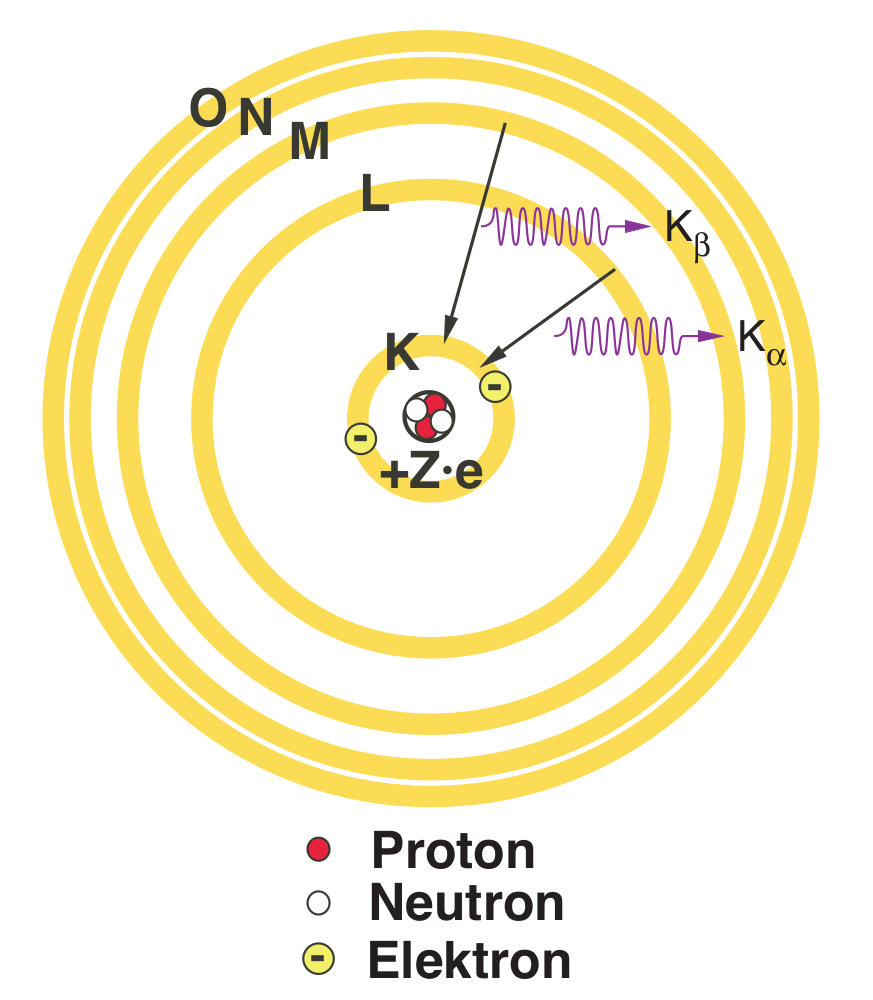
\includegraphics[width=0.95\textwidth]{images/charakt-strahlung.png}
    \captionof{figure}{%
        Schema der Emittierung von charakteristischen Photonen \emph{Quelle}: Versuchsanleitung
    }
    \label{fig:charaktStrahlung}
%\end{figure}
\end{minipage}

Die beiden K-Linien dominieren dabei das Spektrum.


% ---------------------------------------------------------------------------- %
\subsection[Beugung von R\"ontgen-Strahlung an Kristallen]{Beugung von R\"ontgen-Strahlung an Kristallen, R\"ontgen-Spektrometer}
\label{subsec:rontgenBeugung}
% ---------------------------------------------------------------------------- %


\begin{minipage}[c][][b]{0.585\textwidth}
    R\"ontgenstrahlen  werden  an  einem   Kristallgitter  gebeugt,  wenn  die
    Bragg'sche Gleichung (Gleichung \ref{eq:bragg}) erf\"ullt ist:

    \begin{equation}
        \label{eq:bragg}
        2 \cdot d \cdot sin \vartheta_n = n \cdot \lambda
    \end{equation}

    Dabei   ist  $d$   der  Netzebenenabstand. Netzebenen   sind  von   Atomen
    regelm\"assig belegte  Ebenen in einer Kristallstruktur,  entsprechen also
    nicht unbedingt den Gitterf\"achen (bzw. $d$ ist nicht unbedingt identisch
    zu einer Gitterkonstanten).

    Abbildung \ref{fig:braggHerleitung}  stellt schematisch das  Einfallen und
    Reflektieren  von  Strahlung  in  und  an  einem  Kristallgitter  und  die
    Netzebenen dar.

    $\vartheta$ ist  der so  genannte \textbf{Glanzwinkel}. Er  beschreibt den
    Winkel zwischen Netzebene und ein- bzw. ausfallendem Strahl.

\end{minipage}
\begin{minipage}[c][][b]{0.4\textwidth}
    \centering
    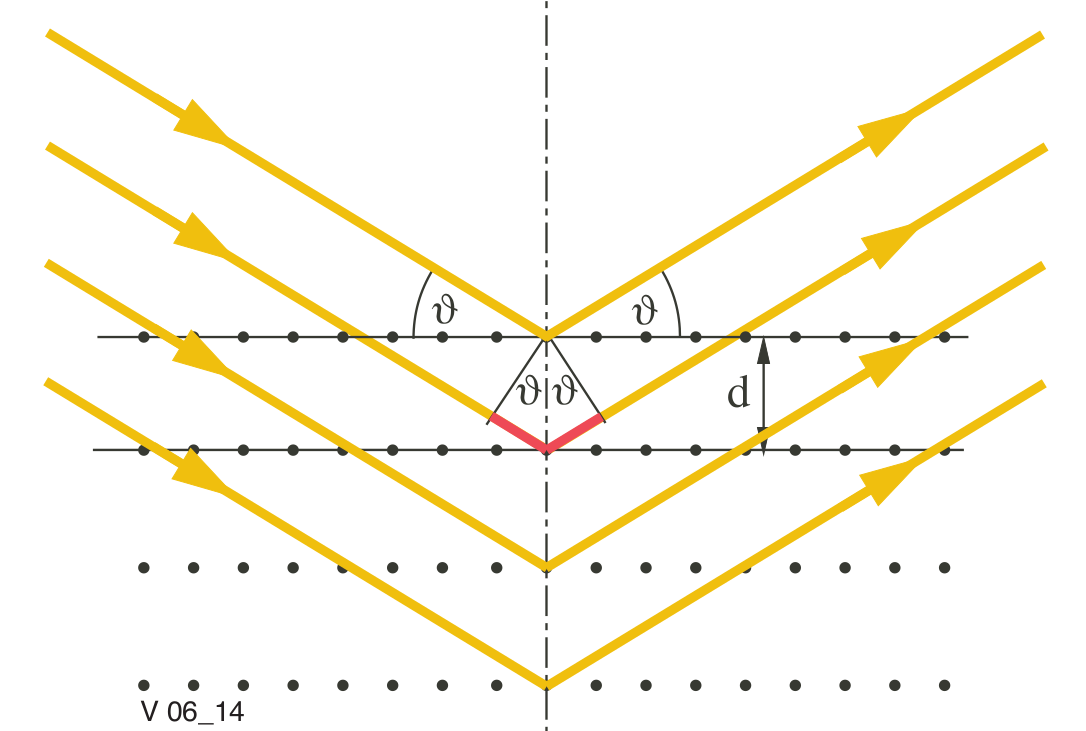
\includegraphics[width=0.95\textwidth]{images/bragg-herleitung.png}
    \captionof{figure}{%
        Schema     zur      Herleitung     der      Bragg'schen     Gleichung.
        \emph{Quelle:} Versuchsanleitung
    }
    \label{fig:braggHerleitung}
\end{minipage}

Es gibt  verschiedene Verfahren, um  sich das R\"ontgenstrahlung  zum Einblick
ins Innere einer  Kristallstruktur zu Nutze zu machen. In  diesem Versuch wird
die \textbf{Bragg'sche Drehkristallmethode} verwendet.

Dabei wird ein  Kristall in einer Halterung rotiert  und mit monochromatischer
Strahlung bestrahlt. Nur  bei bestimmten Winkeln  wird der Strahl  am Kristall
reflektiert und im Z\"ahlrohr detektiert (siehe Abbildung \ref{fig:braggDrehkristall}

\begin{figure}[h!]
    \centering
    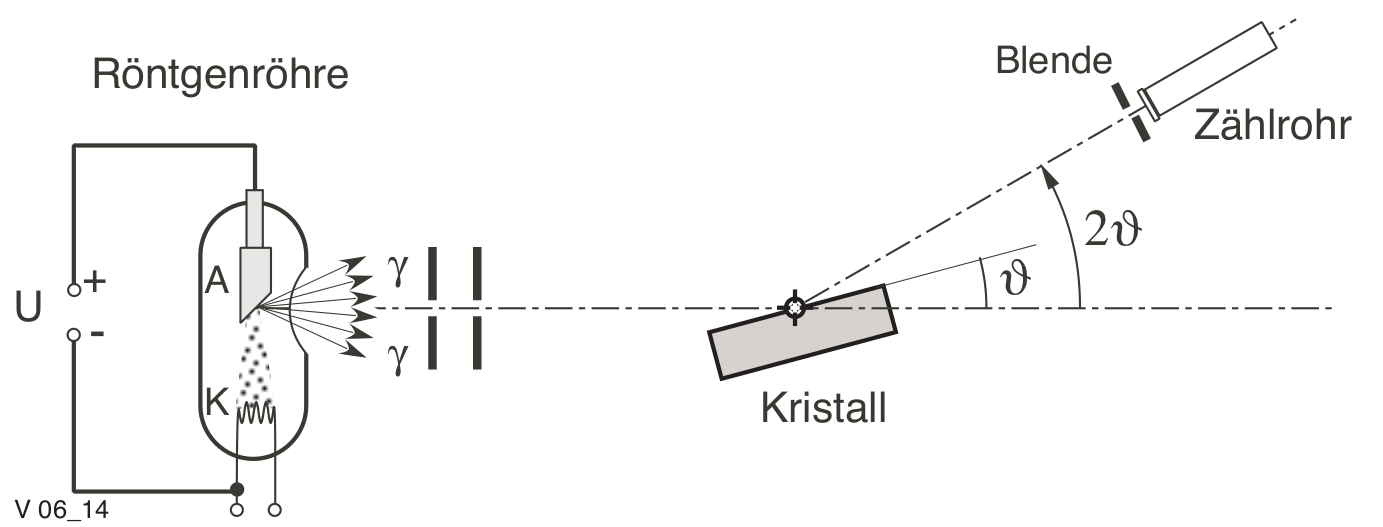
\includegraphics[width=0.5\textwidth]{images/bragg-drehkristall.png}
    \caption{%
        Schema der Versuchsanordnung
        \emph{Quelle:} Versuchsanleitung
    }
    \label{fig:braggDrehkristall}
\end{figure}

